\section{Application context}

\begin{frame}{Corpus}
    
    \begin{itemize}
        \item Over $1.1$ million Document Families
        \item Over $127.8$ millions individual documents
        \item $25$ languages
        \item Documents' texts contain average $50$ characters and $7$ words
        \item Over $210$ thousand tags, amongst which:
        \begin{itemize}
            \item Over $2.5$ thousand suppliers and manufacturers
            \item Over $1.9$ thousand catalogues
            \item Over $208$ thousand categories
        \end{itemize}
    \end{itemize}

    Some text content examples are:
    \begin{itemize}
        \item \emph{DIN 912}
        \item \emph{The P01 to P08 pumps are designed to pump lubricating fluids (oil, diesel oil, etc.). Their flow rate is from 1 to 24 L / min; maximum working pressure 10 bar.} 
    \end{itemize}

\end{frame}

\begin{frame}{User searches}
    
    User text searches:
    \begin{itemize}
        \item are composed of domain-specific keywords, notations, identifiers, and
        acronyms.
        \item contain on average 13 characters separated into 2 words.
        \item can come in any languages
    \end{itemize}

    Some common search examples are:
    \begin{center}
        \emph{motor}, \emph{din 912}, and \emph{ball valve}.
    \end{center}
    
\end{frame}

\begin{frame}{Traceparts search system challenges}
    
    Traceparts search challenges come from:
    \begin{itemize}
        \item Short multilingual texts
        \item Technical texts with many synonyms, acronyms, homonyms, and notations
        \item A large and heterogeneous corpus
        \item Multiple engineering domains coverage
        \item High recall but low precision
    \end{itemize}

\end{frame}

\begin{frame}{Traceparts search system}
    
    \begin{center}
        A text-based search engine.
    \end{center}
    
    \begin{figure} [H]
        \begin{center}
            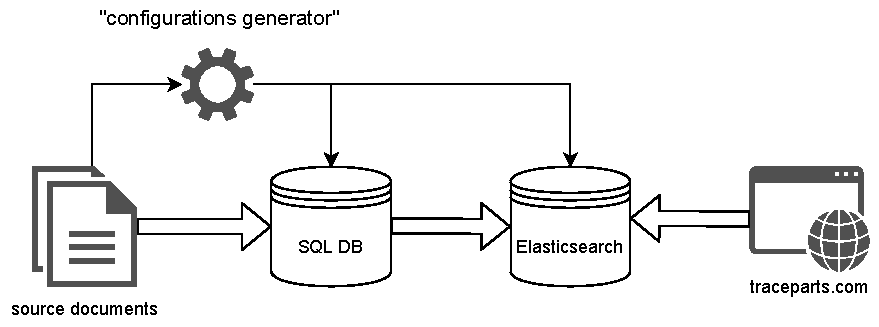
\includegraphics[scale=0.7]{images/tp_system.pdf} 
            \caption{Traceparts current system} 
        \end{center}
    \end{figure}

    \begin{center}
        Parts configurations are generated with their text content to be searchable.    
    \end{center}
    
\end{frame}